\documentclass{article}
\usepackage{amsmath}
\usepackage{amsfonts}
\usepackage{graphicx} % Required for inserting images
\graphicspath{ {./images/} }
\usepackage{mathtools}
\allowdisplaybreaks

\mathtoolsset{showonlyrefs}

\title{FYP}
\author{Johns Noble}
\date{January 2025}

\begin{document}

\maketitle

\newpage
\tableofcontents
\newpage

\section{Introduction}
\subsection{Solving Inhomogenous PDEs}
We will begin by considering an equation in the form of $\mathcal{D}u=f$.
The green's function for a particular PDE is defined in a way such that for a green's function $G(x,x')$ given for some differential operator $\mathcal{D}$, we have that $\mathcal{D}G(x,x') = \delta(x,x')$
My project will be to go through how we can quickly and efficiently by decomposing into orthogonal polynomials and then utilising the recurrence properties of these OPs to solve PDEs using a Dynamic Programming approach.
\subsection{Cauchy Transform}
\begin{equation} \label{cauchy transform}
C_\Gamma f(z):=\frac{1}{2\pi i}\int_\Gamma \frac{f(t)}{t-z}dt
\end{equation}
This is analytic for $z \not\in \Gamma$. Define Hilbert Transform to be the limits from the right and the left.
\subsection{Orthogonal Polynomials}
\begin{center}
\begin{tabular}{ |c|c|c|c| } 
 \hline
	Family & Notation & Interval & $w(x)$ \\ 
 \hline
	Legendre & $P_n(x)$ & [-1,1] & $1$ \\ 
	Chebyshev (1st) & $T_n(x)$ & [-1,1] & $(1-x^2)^{-1/2}$ \\ 
	Chebyshev (2nd) & $U_n(x)$ & [-1,1] & $(1-x^2)^{1/2}$ \\
	Ultraspherical & $C_n^{(\lambda)}(x),\:\lambda>-\frac{1}{2}$ & [-1,1] & $(1-x^2)^{\lambda-1/2}$ \\
	Jacobi & $P_n^{(\alpha,\beta)}(x),\:\alpha,\beta>-1$ & [-1,1] & $(1-x)^\alpha(1-x)^\beta$ \\
 \hline
\end{tabular}
\end{center}
\section{Log and Stieltjes Transform}
In this section we will consider approaches to compute these weakly singular integrals
$$ \int_Alog||z-t||f(t)dt \qquad \int_A\mathbf{\nabla}log||z-t||f(t)dt $$
\begin{equation}\label{stieltjes transform}
	\mathcal{S}_Af(z):= \int_A\frac{f(t)}{z-t}dt \\
\end{equation}
\begin{equation}\label{log transform}
	\mathcal{L}_Af(z):= \int_Alog(z-t)f(t)dt
\end{equation}
Depending on the type of area which $A$ is we can begin by approximating $f$ using orthogonal polynomials.
\subsection{Transforms across Intervals}
We will try to formulate recurrence relations for these transforms across interval [-1, 1].
We are looking for looking for $\mathcal{S}_{[-1,1]}f(z)$.
Decomposing $f(z) \approx \Sigma_k f_kP_k(z)$ and writing $S_k(z):=\mathcal{S}_{[-1,1]}P_k(z)$ lets us write:
$$\mathcal{S}_{[-1,1]}f(z) \approx \Sigma_k f_kS_k(z)$$
This motivates finding fast methods to compute $S_k(z)$. Log kernels are approached similarly letting $L_k(z):=\mathcal{L}_{[-1,1]}P_k(z)$ and looking for recurrence relations.
\subsubsection{Stieltjes kernel on interval}
Recall recurrence relation of Legendre Polynomials:
\begin{equation}\label{legendre recurrence}
	xP_k(x) = \frac{k}{2k+1}P_{k-1}(x) + \frac{k+1}{2k+1}P_{k+1}(x)
\end{equation}
Formulate three-term recurrence for their Stieltjes transforms.
\begin{equation}
\begin{split}
	zS_k(z) &= \int_{-1}^{1}\frac{zP_k(t)}{z-t}dt \\
	&= \int_{-1}^{1}\frac{z-t}{z-t}P_k(t)dt+\int_{-1}^{1}\frac{tP_k(t)}{z-t}dt \\
	&= \int_{-1}^{1}P_k(t)dt+\frac{k}{2k+1}\int_{-1}^{1}\frac{P_{k-1}(t)}{z-t}dt+\frac{k+1}{2k+1}\int_{-1}^{1}\frac{P_{k+1}(t)}{z-t}dt \\
	&= 2\delta_{k0}+\frac{k}{2k+1}S_{k-1}(z)+\frac{k+1}{2k+1}S_{k+1}(z) \\
	S_0(z) &= \int_{-1}^{1}\frac{dt}{z-t} = log(z+1)-log(z-1)
\end{split}
\end{equation}
We can extend this to work over a square using the recurrence over intervals:
\begin{equation}
\begin{split}
zS_{k,j}(z) &= z\int_{-1}^1\int_{-1}^1\frac{P_k(s)P_j(t)}{z-(s+it)}dsdt \\
&= \int_{-1}^1zP_j(t)\int_{-1}^1\frac{P_k(s)}{z-it-s}dsdt \\
&= \int_{-1}^1(z-it)P_j(t)S_k(z-it)+itP_j(t)S_k(z-it)dsdt \\
&= \int_{-1}^1P_j(t)(\frac{k}{2k+1}S_{k-1}(z-it)+\frac{k+1}{2k+1}S_{k+1}(z-it)+2\delta_{k0}) \\
&+i(\frac{j}{2j+1}P_{j-1}(t)+\frac{j+1}{2j+1}P_{j+1}(t))S_k(z-it)dsdt \\
&= \frac{k}{2k+1}S_{k-1,j}(z)+\frac{k+1}{2k+1}S_{k+1,j} \\
&+i\frac{j}{2j+1}S_{k,j-1}(z)+i\frac{j+1}{2j+1}S_{k,j+1}+4\delta_{j0}\delta{k0}
\end{split}
\end{equation}
\subsubsection{Log kernel on interval}
We can begin by connecting log kernel to the Stieltjes kernel. To do this we define:$$S_k^{(\lambda)}(z):=\int_{-1}^{1}\frac{C_k^{(\lambda)}(t)}{z-t}dt$$
We let $F(x) = \int_x^1f(s)ds$ and apply integration by parts on log transform:
\begin{equation}
\begin{split}
	\int_{-1}^1f(t)log(z-t)dt &= [-F(t)log(z-t)]_{-1}^1-\int_{-1}^1\frac{F(t)}{z-t}dt \\
	&= log(z+1)\int_{-1}^1f(t)dt-\int_{-1}^1\frac{F(t)}{z-t}dt
\end{split}
\end{equation}

Since $C_1^{(-1/2)}(x)=-x$ and $\int_x^1P_0(s)ds = 1-x$ we make an adjustment for the case $k=0$:
$$\int_x^1P_k(s)ds = \delta_{k0}+C_{k+1}^{(-1/2)}(x)$$
Also because $\int_{-1}^1P_k(s)ds=2\delta_{k0}$:
\begin{align}
    L_k(z)&=log(z+1)\int_{-1}^1P_k(s)ds-\int_{-1}^1\frac{1}{z-t}\int_t^1P_k(s)dsdt\\
    &=2log(z+1)\delta_{k0}-\int_{-1}^1\frac{C_{k+1}^{(-1/2)}(t)}{z-t}+\frac{\delta_{k0}}{z-t}dt\\
    &=2log(z+1)\delta_{k0}-S_{k+1}^{(-1/2)}(z)-\int_{-1}^1\frac{\delta_{k0}}{z-t}dt\\
    &=-S_{k+1}^{(-1/2)}(z)+\delta_{k0}((z-1)log(z-1)+(z+1)log(z+1))
\end{align}
Now we employ the recurrence relation of $C_{k}^{(-1/2)}$ to solve for the recurrence relation of $L_k(s)$:
\begin{align}
    tC_k^{(\lambda)}(t)&=\frac{k+2\lambda-1}{2(k+\lambda)}C_{k-1}^{(-1/2)}(t)+\frac{k+1}{2(k+\lambda)}C_{k+1}^{(-1/2)}(t)\\
    tC_k^{(-1/2)}(t)&=\frac{k-2}{2k-1}C_{k-1}^{(-1/2)}(t)+\frac{k+1}{2k-1}C_{k+1}^{(-1/2)}(t)
\end{align}
Following the process of introducing a multiple of $z$ and decomposing into $z-t,t$ as we did for $S_k$ yields the following function recurrence:
\begin{align}
    zL_k(z)&=\frac{k-1}{2k+1}L_{k-1}(z)+\frac{k+2}{2k+1}L_{k+1}(z)\\
    &+\begin{cases}
	(z-1)log(z-1)+(z+1)log(z+1),&k=0\\
	-2/3,&k=1\\
	0,&\text{otherwise}
    \end{cases}
\end{align}

\subsection{Log kernel interval linear transformations}
Now that we have a recurrence relation of the log kernel on a simple interval, we will try and formulate a way to extend this to work on linearly transformed intervals.
The motivation to do this will become clear later on when we attempt to use boundary element methods to help solve a poisson PDE.
Let us aim to be able to scale and rotate by some $\lambda$ and move by some $\mu$.
\begin{align}
    L_k(z)=\int_{-1}^1P_k(s)&Log(z-s)ds\rightarrow\int_{-1}^1P_k(s)Log(z-(\mu+\lambda s))ds\\
    \int_{-1}^1P_k(s)log(z-\mu-\lambda s)ds&=\int_{-1}^1P_k(s)log(\lambda(\frac{z-\mu}{\lambda}-s))ds
\end{align}
From here we have to be careful with considering branch cuts.
The idea is that we have an interval which is moved by $-\mu$ from our $z$ and going up direction $-\lambda$ as we go from $-1\rightarrow 1$.
Thinking about flat interval we think about what occurs when this is rotated clockwise by angle $\lambda$.

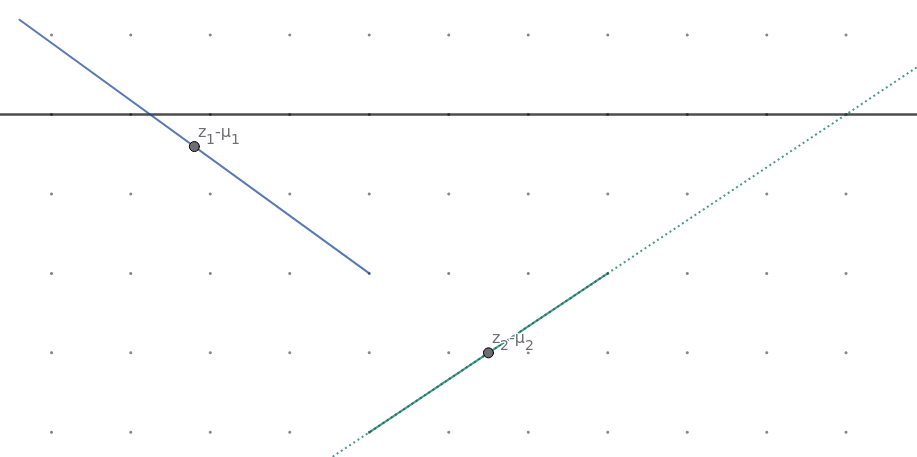
\includegraphics[width=\textwidth]{intervaltransform}

Above is a small example where we can see what the interval in the integral we are trying to decompose the log of looks like.
We see here are that we may already have a cut crossing which means it is important to know at what value of $s$, this crossing occurs and then trelike two seperate integrals.
Now we are able to rotate and see that it will lie entirely above or below the branch cut as it is flat.
We can imagine in the image above the origin being at different points along the real axis.
If we try mentally rotate these intervals around any chosen origin point along this real axis, we will find that when the extended line in the direction of $\lambda$ intercepts the real axis, we have a branch crossing given that the this intersection happens in the negative region of the line.
TODO: Prove this statement
We can find intercept at the real axis fairly easily to be:
\begin{align}
    Im:\:Im(z-\mu-\lambda s^*)&=0\\
    Im(z-\mu)&=Im(\lambda)s^*\implies s^*=\frac{Im(z-\mu)}{Im(\lambda)}\\
    x^*=Re(z-\mu-\lambda s^*)&=Re(z-\mu)-s^*Re(\lambda)=Re(z-\mu)-\frac{Im(z-\mu)Re(\lambda)}{Im(\lambda)}
\end{align}
If $s^*>1$ then it means there is no point in the direction of $\lambda$ which intersects the real axis which means we do not have to make any corrections.
Provided it holds that $s^*<1$, if there is an $x^*\geq 0$ then we have no correction.
Otherwise we handle the correction based on the direction we are rotating in:
\begin{align}
    C(s)=\begin{cases}
	0,&arg(\lambda)=0\text{ or }s^*>1\text{ or }x^*\geq 0\\
	-2\pi i\mathbb{I}\{s>s^*\},&arg(\lambda)>0\\
	2\pi i\mathbb{I}\{s<s^*\},&arg(\lambda)<0
    \end{cases}
\end{align}
Revisiting earlier, we can show say that our transformed version is like:
\begin{align}
    \int_{-1}^1P_k(s)log(\lambda(\frac{z-\mu}{\lambda}-s))ds&=\int_{-1}^1P_k(s)(log(\lambda)+log(\frac{z-\mu}{\lambda}-s)+C(s))ds\\
    &=2log(\lambda)\delta_{k0}+L_k(\frac{z-\mu}{\lambda})+\int_{-1}^1P_k(s)C(s)ds
\end{align}

\section{Stieltjes Polynomial Transforms}
We can begin to consider taking these transforms across different geometries.
Currently we have a way to find these transforms across [-1,1] but we will be trying to use this to solve other geometries.
The first type of geometry we should consider is one where we apply a degree $d$ polynomial transform to the interval:
$$p:[-1,1]\rightarrow \Gamma$$
We will show why the solution to a cauchy transform across this interval is as follows:
\begin{equation}
C_\Gamma f(z) = \Sigma_{j=0}^dC_{[-1,1]}[f\circ p](p_j^{-1}(z))
\end{equation}
Where $p_j^{-1}(z)$ are the $d$ pre-images of $p$.
In order to solve this we will use plemelj.
There are 3 properties that need to hold for a function $\psi: \Gamma \rightarrow \mathbb{C}$ to be a cauchy transform:
\begin{equation}\label{cauchy_conditions}\begin{gathered}
\underset{z\to\infty}{lim}= 0 \\
\psi^+(z)-\psi^-(z)= f(z) \\
\psi\;analytic\;on\;\Gamma 
\end{gathered}\end{equation}

Checking \eqref{cauchy_conditions}.1 we get that $\underset{z\to\infty}{p_j^{-1}(z)} = \infty \implies$
\begin{equation}\begin{split}
\underset{z\to\infty}{lim}C_\Gamma f(z) &= \Sigma_{j=1}^d \underset{z\to\infty}{lim}C_{[-1,1]}(f\circ p)(p_j^{-1}(z)) \\
&= \Sigma_{j=1}^d C_{[-1,1]}(f\circ p)(\underset{z\to\infty}{lim} p_j^{-1}(z)) \\
&= \Sigma_{j=1}^d 0 = 0
\end{split}\end{equation}

Checking \eqref{cauchy_conditions}.2 we need an expression for $\psi^+$ and $\psi^-$.
Let us begin by saying that we are looking for cauchy transform of point $s$ which happens to lie on $\Gamma$.
This means that there is a unique root of $t_k := p_k^{-1}(s) \in [-1,1]$.
TODO: Show that $\underset{z\to s^+}{lim} p_k^{-1}(s) =\underset{z\to p^{-1}(s)^+}{lim}$.
Taking limits of $\psi^+, \psi^-$ gives us:
\begin{equation}\begin{split}
\psi^+(s)&=\underset{z\to s}{lim}\:C_{[-1,1]}(f\circ p)(p_k^{-1}(z)) \\
&+\Sigma_{j\neq k}C_{[-1,1]}(f\circ p)(p_j^{-1}(s)) \\
&=C^+_{[-1,1]}(f\circ p)(p_k^{-1}(z)) \\
&+\Sigma_{j\neq k}C_{[-1,1]}(f\circ p)(p_j^{-1}(s)) \\
\end{split}\end{equation}
We can do a similar thing with $\psi^-$ and putting everything together:
\begin{equation}\begin{split}
\psi^+(s)-\psi^-(s)&=C_{[-1,1]}^+(f\circ p)(p_k^{-1}(s))-C_{[-1,1]}^-(f\circ p)(p_k^{-1}(s)) \\
&= (f\circ p)(p_k^{-1}(s)) = f(s)
\end{split}\end{equation}
In the case where $z \notin \psi, \psi^+=\psi^-$ which is expected since the area in between is analytic

TODO show that condition \eqref{cauchy_conditions}.3 holds
\section{Affine Transformations}
Affine transformations can be solved in 2 distinct ways:
We will begin by considering the case of solving for a horizontally skewed square with the following transformation:
$$\begin{pmatrix}x\\y\end{pmatrix}\rightarrow
\begin{pmatrix}\alpha x+\beta y\\y\end{pmatrix}$$
It can be shown that any affine transformation in the form of $(x, y)^T \rightarrow A(x,y)^T$ can be done by taking the above translation and performing scaling and rotations.
TODO: Show that this is indeed the case

\section{Trapezium Region}
We can attempt to generalise the method of stieltjes on a square to work for any given quadrilateral.
This can easily be done by computing for a Trapezium,
We can use the parameterisation: $$Q\begin{pmatrix}x\\y\end{pmatrix}\rightarrow
\begin{pmatrix}(1+x)(\alpha+\beta y)\\y\end{pmatrix}$$
Since our $\alpha, \beta > 0$, our $Q$ is invertible:
$$Q^{-1}\begin{pmatrix}s\\t\end{pmatrix}\rightarrow\begin{pmatrix}\frac{s}{\alpha+\beta t}-1\\t\end{pmatrix}$$

There are two approaches which were considered which vary in which functions we are using for our bases.
The first approach that was attempted would be to take the function approximation as follows:
$$f(x,y)=\Sigma_{k,j}c_{k,j}P_k(x)P_j(y), c_{k,j}\in \mathbb{R}$$
This method is simpler but it can be seen that we would have to be evaluating integrals of orthogonal polynomials outside the
$[-1,1]$ domain in which they are well behaved.
This would result in instable results

It is possible to think of the function space here as the bases of functions which we can add together to approximate the function.
In the approach above we can represent the bases to be $\{b_{kj}\}_{kj}$ where $b_{kj}(\textbf{x})=P_k(x)P_j(y)$
The approach we will focus on here is the approximation following taking an approximation using the function bases as follows:
\begin{align}
    f\circ Q(x,y) &= \Sigma_{k,j}c_{k,j}P_k(x)P_j(y),\:c_{k,j}\in \mathbb{R}\\
    f\circ Q(\textbf{x})&=\Sigma_{k,j}c_{k,j}b_{kj}(\textbf{x})\\
    Q\:invertible \implies
    f(\textbf{x})&=\Sigma_{k,j}c_{k,j}b_{kj}(Q^{-1}(\textbf{x}))
\end{align}
This means we have an altered set of basis based on $\alpha,\beta$ where the new basis can be represented as:
$$\{\tilde{b}_{kj}=b_{kj}\circ Q^{-1}\}_{kj}$$
In this approach we are need to be able to compute $$s_{kj}:=\int_{-1}^1 (\alpha+\beta t) \int_{-1}^1 \frac{P_j(t)P_k(s)}
{z-it-(\alpha+\beta t)(1+s)} ds dt$$
As you can see here there is a term in the denominator which is difficult to deal with as it is harder to seperate the $s$ and $t$ terms.
In order to begin we come up with a few different rearrangements of this equation:
\begin{align}
\tilde{s_{kj}} :&= \int_{-1}^1 \int_{-1}^1 \frac{P_j(t)P_k(s)}
{z-it-(\alpha+\beta t)(1+s)} ds dt\\
&= \int_{-1}^1\frac{1}{\alpha+\beta t}\int_{-1}^1 \frac{P_j(t)P_k(s)}
{\frac{z-it}{\alpha+\beta t}-1-s}dsdt\\
&=: \int_{-1}^1\frac{P_j(t)}{\alpha+\beta t}\int_{-1}^1 \frac{P_k(s)}{\tilde{z_t}-s} \\
\tilde{s_{kj}} &= \int_{-1}^1\int_{-1}^1
\frac{P_j(t)P_k(s)}{z-\alpha(1+s)-(i+\beta(1+s))t}dsdt \\
&= \int_{-1}^1\frac{P_k(s)}{\beta(1+s)+i}\int_{-1}^1 \frac{P_j(t)}{
	\frac{z-\alpha(1+s)}{\beta(1+s)+i}-t}dtds\\
&= \int_{-1}^1\frac{P_k(s)}{\beta(1+s)+i}\int_{-1}^1 \frac{P_j(t)}{
\tilde{z_s}-t}dtds\\
\end{align}

Here, I've used $\tilde{z_t}$ and $\tilde{z_s}$ to denote different constants although rigorously both are actually two different functions.
It is always the case where $\tilde{z_t}, \tilde{z_s}$ denotes
$\frac{z-it}{\alpha+\beta t}-1,\frac{z-\alpha(1+s)}{\beta(1+s)+i}$ respectively

It is also very useful to define function $s_k, s_j$:
\begin{align}
	s_k(z) :&= \int_{-1}^1\frac{P_k(s)}{z-s}ds \\ 
	s_j(z) :&= \int_{-1}^1\frac{P_j(t)}{z-t}dt \\ 
\end{align}

This can be motivated by the tricky recurrent forms for $\tilde{s_{k0}}$.
TODO: Show why tricky?

We can recreate $s_{kj}$ using values of $\tilde{s_{kj}}$ by doing the following:
\begin{align}
	let\; I(k,j,s,t) :&= \frac{P_j(t)P_k(s)}{z-it-(\alpha+\beta t)(1+s)}\\ 
	s_{kj} &= \int_{-1}^1(\alpha+\beta t)\int_{-1}^1 I(k,j,s,t) dsdt\\
	&= \int_{-1}^1\alpha\int_{-1}^1 I(k,j,s,t)dsdt +
	\int_{-1}^1\beta t\int_{-1}^1 I(k,j,s,t) dsdt\\
	&= \alpha\tilde{s_{kj}} + \beta\frac{j}{2j+1}\tilde{s_{kj-1}} + \beta\frac{j+1}{2j+1}\tilde{s_{kj+1}} \\
	s_{k0} &= \int_{-1}^1\alpha\int_{-1}^1 I(k,0,s,t)dsdt +
	\int_{-1}^1\beta t\int_{-1}^1 I(k,0,s,t) dsdt \\
	&= \alpha\tilde{s_{k0}} + \beta\tilde{s_{k1}}
\end{align}

\subsection{Recurrences}

Now we can go about trying to construct these recurrences.
To make it easier notationally to represent these legendre recurrence relations, it is convenient to represent it as the following:
\begin{align}
    xP_j(x) &= \frac{j}{2j+1}P_{j-1}(x)+\frac{j+1}{2j+1}P_{j+1}(x) \\
    &:= j_-P_{j-1}(x)+j_+P_{j+1}(x)
\end{align}
It is easiest to begin with a case where:

\subsubsection{Case 1: $k,j>1$}

\begin{align}
	z\tilde{s_{kj}}&=\int_{-1}^1z\frac{P_j(t)}{\alpha+\beta t}s_k(\tilde{z_t})dt\\
	&=\int_{-1}^1P_j(t)\frac{z-it}{\alpha+\beta t}s_k(\tilde{z_t})dt
	+\int_{-1}^1\frac{itP_j(t)}{\alpha+\beta t}s_k(\tilde{z_t})dt\\
	&=\int_{-1}^1P_j(t)\tilde{z_t}s_k(\tilde{z_t})dt
	+\int_{-1}^1P_j(t)s_k(\tilde{z_t})
	+\int_{-1}^1\frac{itP_j(t)}{\alpha+\beta t}s_k(\tilde{z_t})dt\\
\end{align}

It is useful here to come up with an expression for:

\begin{align}
    \int_{-1}^1P_j(t)s_k(\tilde{z_t}) &= \int_{-1}^1(\alpha+\beta t)\frac{P_j(t)}{\alpha + \beta t} s_k(\tilde{z_t})dt\\
    &= \int_{-1}^1\frac{\alpha P_j(t)}{\alpha+\beta t}s_k(\tilde{z_t})dt+\int_{-1}^1\frac{\beta tP_j(t)}{\alpha+\beta t}s_k(\tilde{z_t})dt\\
    &= \alpha\tilde{s_{kj}} + \beta j_-\tilde{s_{kj-1}}+\beta j_+\tilde{s_{kj+1}}
\end{align}

Similarly:
\begin{align}
    \int_{-1}^1P_k(s)s_j(\tilde{z}_s)ds &= \int_{-1}^1(\beta(1+s)+i)\frac{P_k(s)}{\beta(1+s)+i}s_j(\tilde{z}_s)ds\\
    &=\int_{-1}^1(\beta+i+\beta s)\frac{P_k(s)}{\beta(1+s)+i}s_j(\tilde{z}_s)ds\\
    &=(\beta+i)\tilde{s}_{kj}+\beta k_-\tilde{s}_{k-1j}+\beta k_+\tilde{s}_{k+1j}
\end{align}

Decomposing individual elements of the previous equation:

\begin{align}
	\int_{-1}^1P_j(t)\tilde{z_t}s_k(\tilde{z_t})dt&=\int_{-1}^1P_j(t)(k_-s_{k-1}(\tilde{z_t})+k_+s_{k+1}(\tilde{z_t}))dt\\
	&= k_-(\alpha\tilde{s_{k-1j}}+\beta j_-\tilde{s_{k-1j-1}}+\beta j_+\tilde{s_{k-1j+1}})\\
	&+ k_+(\alpha\tilde{s_{k+1j}}+\beta j_-\tilde{s_{k+1j-1}}+\beta j_+\tilde{s_{k+1j+1}})\\
	\int_{-1}^1P_j(t)s_k(\tilde{z_t}) &= \alpha\tilde{s_{kj}} + \beta j_-\tilde{s_{kj-1}}+\beta j_+\tilde{s_{kj+1}}\\
	\int_{-1}^1\frac{itP_j(t)}{\alpha+\beta t}s_k(\tilde{z_t})dt &= i(j_-\tilde{s_{kj-1}}+j_+\tilde{s_{kj+1}})
\end{align}

Returning back to our original equation:

\begin{align}
    z\tilde{s_{kj}}&=\int_{-1}^1P_j(t)\tilde{z_t}s_k(\tilde{z_t})dt
    +\int_{-1}^1P_j(t)s_k(\tilde{z_t})
    +\int_{-1}^1\frac{itP_j(t)}{\alpha+\beta t}s_k(\tilde{z_t})dt\\
    &=\beta(k_-j_-\tilde{s}_{k-1j-1}+k_-j_+\tilde{s}_{k-1j+1}+k_+j_-\tilde{s}_{k+1j-1}+k_+j_+\tilde{s}_{k+1j+1})\\
    &+\alpha(\tilde{s}_{kj}+k_-\tilde{s}_{k-1j}+k_+\tilde{s}_{k+1j})\\
    &+(\beta+i)(j_-\tilde{s}_{kj-1}+j_+\tilde{s}_{kj+1})
\end{align}

The decision to have $t$ as the outside integral was completely arbritary, we could have taken $s$ as the outside integral and we would have reached the exact same recurrence relation.
We can see that for a log kernel we would have different relations which we can use in our benefit to skip finding certain base cases.

And thus we have a 9 point stencil recurrence relation.
Given any 8 points we are able to find the final point.
Assuming we therefore for some $k,j\geq 2$ we have all $\tilde{s}_{nm}$ for all $n\leq k,m\leq j$,
we can compute the value of $\tilde{s}_{k+1j+1}$ since we other values $mn$ centered around $kj$.
Now we need a way of finding the base case, in particular, the case of the two initial rows and columns.

To begin with the computations of the $k=1,j=1$ rows/cols, it is useful to prove the following:
\begin{align}
    zs_0(z)&=\int_{-1}^1\frac{z}{z-s}ds \\
    &= \int_{-1}^11+\frac{s}{z-s}ds\\
    &= 2+s_1(z)
\end{align}

\subsubsection{Case 2: $k=1$}
For this we are going to assume that we already have values of the following: $\tilde{s}_{kj}$ where both $k\leq1 \wedge j\leq1$ as well as for all $k=0$ and $j=0$.
Computation of these will be another case outlined later.
We are able to find a 6 point stencil relation by first beginning with the expansion for $z\tilde{s}_{0j}$
\begin{align}
    z\tilde{s}_{0j}&=\int_{-1}^1\frac{zP_j(t)}{\alpha+\beta t}s_0(\tilde{z}_t)dt\\
    &= \int_{-1}^1P_j(t)\frac{z-it}{\alpha+\beta t}s_0(\tilde{z}_t)dt
    +\int_{-1}^1\frac{itP_j(t)}{\alpha+\beta t}s_0(\tilde{z}_t)dt\\
    &= \int_{-1}^1P_j(t)\tilde{z}_ts_0(\tilde{z}_t)dt
    +\int_{-1}^1P_j(t)s_0(\tilde{z}_t)dt
    +\int_{-1}^1\frac{itP_j(t)}{\alpha+\beta t}s_0(\tilde{z}_t)dt\\
    &= \int_{-1}^1P_j(t)(2+s_1(\tilde{z}_t))dt
    +\alpha \tilde{s}_{0j}+\beta j_-\tilde{s}_{0j-1}+\beta j_+\tilde{s}_{0j+1}
    +i j_-\tilde{s}_{0j-1}+i j_+\tilde{s}_{0j+1}\\
    &=4\delta_{0j}+\alpha(\tilde{s}_{0j}+\tilde{s}_{1j})
    +\beta j_-(\tilde{s}_{0j-1}+\tilde{s}_{1j-1})+\beta j_+(\tilde{s}_{0j+1}+\tilde{s}_{1j+1})\\
    &+i j_-\tilde{s}_{0j-1}+i j_+\tilde{s}_{0j+1} \\
    &=4\delta_{0j}+\alpha(\tilde{s}_{0j}+\tilde{s}_{1j})
    +(\beta+i)(j_-(\tilde{s}_{0j-1}+\tilde{s}_{1j-1})+j_+(\tilde{s}_{0j+1}+\tilde{s}_{1j+1}))
\end{align}

\subsubsection{Case 3: $j=1$}
We can use a similar approach for expansion on $z\tilde{s}_{k0}$:
\begin{align}
    z\tilde{s}_{k0} &= \int_{-1}^1\int_{-1}^1\frac{zP_k(s)}{z-it-(\alpha+\beta t)(1+s)}dsdt\\
    &=\int_{-1}^1\frac{zP_k(s)}{\beta(1+s)+i}\int_{-1}^1\frac{1}{\tilde{z}_s-t}dtds\\
    &=\int_{-1}^1\frac{zP_k(s)}{\beta(1+s)+i}s_0(\tilde{z}_s)ds\\
    &=\int_{-1}^1\frac{(z-\alpha(1+s))P_k(s)}{\beta(1+s)+i}s_0(\tilde{z}_s)ds
    +\int_{-1}^1\frac{\alpha(1+s)P_k(s)}{\beta(1+s)+i}s_0(\tilde{z}_s)ds\\
    &=\int_{-1}^1P_k(s)\tilde{z}_ss_0(\tilde{z}_s)ds
    +\int_{-1}^1\frac{\alpha(1+s)P_k(s)}{\beta(1+s)+i}s_0(\tilde{z}_s)ds\\
    &=\int_{-1}^1P_k(s)(2+s_1(\tilde{z}_s))ds+\alpha(\tilde{s}_{k0}+k_-\tilde{s}_{k-10}+k_+\tilde{s}_{k+10})\\
    &=(\beta+i)\tilde{s}_{k1}+\beta k_-\tilde{s}_{k-11}+\beta k_+\tilde{s}_{k+11}
    +\alpha(\tilde{s}_{k0}+k_-\tilde{s}_{k-10}+k_+\tilde{s}_{k+10})\\
\end{align}

\subsubsection{Issue with branch cuts}
For the following cases we are forced to manipulate integral expressions involving logs.
We will be using the log decomposition formula $log(ab)=log(a)+log(b)$.
To highlight our issue lets imagine taking the integral:
$$\int_{0}^1 f(x)log(abx)dx,\:arg(a)+arg(b)>\frac{\pi}{2}$$
Here we see that if we try and decompose $log(abx)$ into $log(ax)+log(b)$,
we will have to add a correction term since
$$arg(abx)\neq (arg(ax)+arg(b)=arg(a)+arg(b)>\frac{\pi}{2})$$
This is because of the branch cut at $\pm\pi$, $arg(abx)=arg(ab)<0$
It is possible to easily fix this by removing a factor of $2\pi$:
$$\int_{0}^1 f(x)log(abx)dx = \int_{0}^1 f(x)log(ax)dx+\int_{0}^1 f(x)(log(b)-2\pi)dx$$

Although this is a very simple case which I am just using to illustrate the point we can get a much more complex case when the interval we are taking integrals over crosses over branch cuts.
To solve this we find the value $w$ such that $arg(z)+arg(w)=\frac{\pi}{2}$:
\begin{align}
    \int_{c_-}^{c_+}f(x)log(zx)dx,&\:arg(z)+arg(c_-)>\frac{\pi}{2}\\
    &arg(z)+arg(c_+)<\frac{-\pi}{2}\\
    \int_{c_-}^{c_+}f(x)log(zx)dx=&\int_{c_-}^wf(x)(log(zx)-2\pi)dx
    +\int_w^{c_+}f(x)log(zx)dx
\end{align}

Before moving to the next two cases we need closed form solutions to the following:

First we define: $$r_j = \int_{-1}^1P_j(t)s_0(\tilde{z}_t)dt$$
It is easy to see here that $r_j = s_{0j}$; we are able to very easily find a recurrence relation for $s_{0j}$:
\begin{align}
    r_j &= \int_{-1}^1P_j(t)s_0(\tilde{z}_t)dt\\
    &=\int_{-1}^1P_j(t)log(\frac{\tilde{z}_t+1}{\tilde{z}_t-1})dt\\
    &=\int_{-1}^1P_j(t)log(\frac{z-it}{z-2\alpha-(2\beta+i)t})dt\\
    &=\int_{-1}^1P_j(t)log(z-it)dt-\int_{-1}^1P_j(t)log(z-2\alpha-(2\beta+i)t)dt\\
    &=\int_{-1}^1P_j(t)log(z-it)dt
    -\int_{-1}^1P_j(t)(log(2\beta+i)+log(\frac{z-2\alpha}{2\beta+i}-t)+C_1(t))dt\\
\end{align}
Where $C_1(t)$ is a correction term as a result of branch cuts from splitting up logs which we will derive later.

We also need to show that it is valid to split up the other logs and prove that there will not exist any branch cuts.
When going through the cases $log(f(t)g(t))$ we are verifying such that for every $t$:
$$|arg(f(t))+arg(g(t))|<\pi$$
First we address:
$$log(\frac{z-it}{z-2\alpha-(2\beta+i)t})$$
We can now consider two cases.
let:
\begin{align}
    z_1&=z-it\\
    z_2&=z-2\alpha-2\beta t-it\\
    k_t&=2\alpha+2\beta t\\
    &\implies (Re(z_1)-k_t, Im(z_1))=(Re(z_2), Im(z_2))
\end{align}
Case 1 ($Im(z_1)=Im(z_2)>0$ - Origin lies below):
\begin{align}
    arg(z_1)+arg(z_2^{-1})&=arg(z_1)-arg(z_2)\\
    arg(z_1)>0,\:arg(z_2)<\pi&\implies arg(z_1)-arg(z_2)>-\pi\\
    arg(z_1)<arg(z_2)&\implies arg(z_1)-arg(z_2)<0
\end{align}
Case 2 ($Im(z_1)=Im(z_2)<0$ - Origin lies above):
\begin{align}
    arg(z_1)+arg(z_2^{-1})&=arg(z_1)-arg(z_2)\\
    arg(z_1)<0,\:arg(z_2)>-\pi&\implies arg(z_1)-arg(z_2)<\frac{\pi}{2}\\
    arg(z_1)>arg(z_2)&\implies arg(z_1)-arg(z_2)>0
\end{align}

In the remaining cases, we have that some values of $t$ is above and some values of $t$ are below which means we can simply combine the logic of these the above two cases to say that there are no issues with branch cuts.

Next we address
$$log(z_2)=log(z-2\alpha-(2\beta+i)t)=log(2\beta+i)+log(\frac{z-2\alpha}{2\beta+i}-t):=log(c_1)+log(z_3)$$

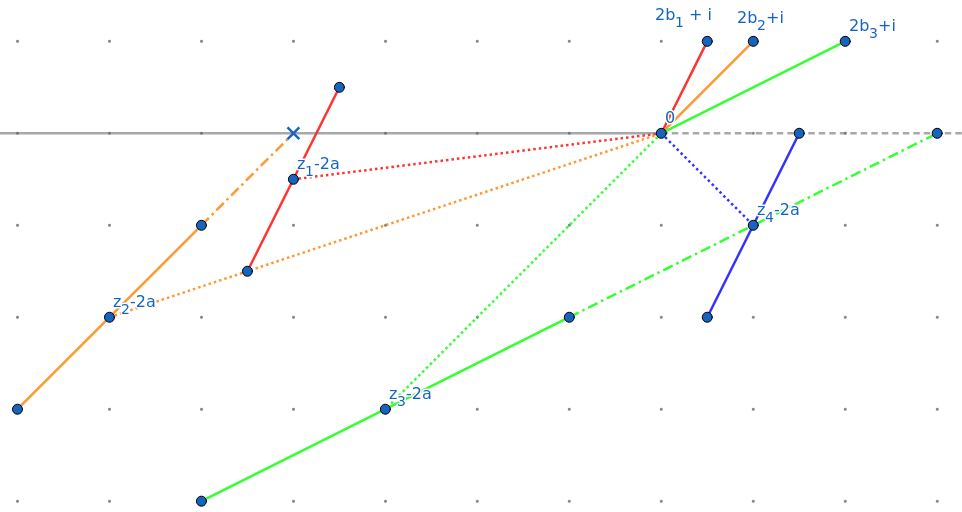
\includegraphics[width=\textwidth]{z23}
The image above helps illustrate how different intervals of $z_2$ look like for various values of $2\beta+i$.
As $b>0$, the $arg(2\beta+i)\in(0,\frac{\pi}{2})$.
Also we note that in $z_3$ the interval is flat.
This should make sense as we have an interval of angle $2\beta+i$ and we are rotating this interval by the same angle.
Therefore the question of branch crossing is reduced down to wether or not the whole interval crosses the line.

Case 1 ($Im(z)>1$):
\begin{align}
    Im(z)>1 &\implies Im(z_2)>1,\:arg(z_2)\in(0,\pi)\\
    arg(2\beta+i)\in(0,\frac{\pi}{2}) &\implies arg(z_3) = arg(z_2)-arg(2\beta + i) \in (-\frac{\pi}{2},\pi)
\end{align}
Case 2 ($arg(z-2\alpha)>-\pi+arg(2\beta+i)$)
Rough idea here is that it is never lifted clockwise over the branch cut.
Again this will be shown using diagrams
Case 3 ($arg(z-2\alpha)<-\pi+arg(2\beta+i)$)
This means the whole interval is lifted over the branch cut.
\begin{align}
    t_1 :&= min\{max\{\underset{t}{inf}\:Im(z-2\alpha-(2\beta+i)t)<0,-1\},1\}\\
    \int_{-1}^1f(t)log(z_2)dt &= \int_{-1}^tf(t)(log(2\beta+i)+log(z_3))dt\\
    &+\int_t^1f(t)(log(2\beta+i)+log(z_3)-2\pi i)dt
\end{align}
Case 4 ($z-2\alpha-2\beta Im(z)>0,\: |Im(z)|\leq 1$):
This is just another way of saying that when parameterising $z_2$ with $t$, the intercept of this line with the real axis is greater than $0$ and so does not pass through the branch cut.
This means we have a case of rotation that does not cross any branch cut (this is because the rotation will result in a flat line).
TODO:Proof for these and diagrams.

Secondly we should also define:
\begin{align}
    q_k&=\int_{-1}^1P_k(s)s_0(\tilde{z}_s)ds\\
    &=\int_{-1}^1P_k(s)log(\frac{\tilde{z}_s+1}{\tilde{z}_s-1})ds
    =\int_{-1}^1P_k(s)log(\frac{z+i-(\alpha-\beta)(1+s)}{z-i-(\alpha+\beta)(1+s)})ds\\
    &=\int_{-1}^1P_k(s)log(z+i-(\alpha-\beta)(1+s))ds\\
    &-\int_{-1}^1P_k(s)log(z-i-(\alpha+\beta)(1+s))ds+\int_{-1}^1C_2(s)ds\\
    &=\int_{-1}^1P_k(s)(log(\alpha-\beta)+log(\frac{z+i}{\alpha-\beta}-1-s))ds\\
    &-\int_{-1}^1P_k(s)(log(\alpha+\beta)+log(\frac{z-i}{\alpha+\beta}-1-s))ds+\int_{-1}^1C_2(s)ds\\
    &=L_k(\frac{z-i}{\alpha-\beta}-1)-L_k(\frac{z-i}{\alpha+\beta}-1)
    +2\delta_{k0}log(\frac{\alpha-\beta}{\alpha+\beta})+\int_{-1}^1C_2(s)ds
\end{align}
In the case where we are attempting to solve over a triangle i.e. $\alpha=\beta$ we have:
\begin{align}
    q_k&=\int_{-1}^1P_k(s)s_0(\tilde{z}_s)\\
    &=\int_{-1}^1P_k(s)log(z+i-(\alpha-\beta)(1+s))ds\\
    &-\int_{-1}^1P_k(s)log(z-i-(\alpha+\beta)(1+s))ds+\int_{-1}^1C_2(s)ds\\
    &=\int_{-1}^1P_k(s)log(z+i)ds-\int_{-1}^1P_k(s)log(z-i-2\alpha(1+s))ds+\int_{-1}^1C_2(s)ds\\
    &=2\delta_{k0}log(z+i)-\int_{-1}^1P_k(s)(log(2\alpha)+log(\frac{z-i}{2\alpha}-(1+s)))ds+\int_{-1}^1C_2(s)ds\\
    &=2\delta_{k0}(log(z+i)-log(2\alpha))-L_k(\frac{z-i}{2\alpha}-1)+\int_{-1}^1C_2(s)ds
\end{align}
First we look for the correction term $C_2$ in the expression:
$$log(\frac{z_4}{z_5})=log(z_4)-log(z_5)$$
$$z_4=z+i-(\alpha-\beta)(1+s),\:z_5=z-i-(\alpha+\beta)(1+s)$$
Case 1 $(Im(z)>1)$:
\begin{align}
    Im(z)>1 &\implies 0<arg(z_4),arg(z_5)<\pi\\
    &\implies |arg(z_4)-arg(z_5)|<\pi
\end{align}
Case 2 $(Im(z)<1)$:
\begin{align}
    Im(z)<1 &\implies -\pi<arg(z_4),arg(z_5)<0\\
    &\implies |arg(z_4)-arg(z_5)|<\pi
\end{align}
For the next 3 cases it is important to understand the geometry of these branch cuts

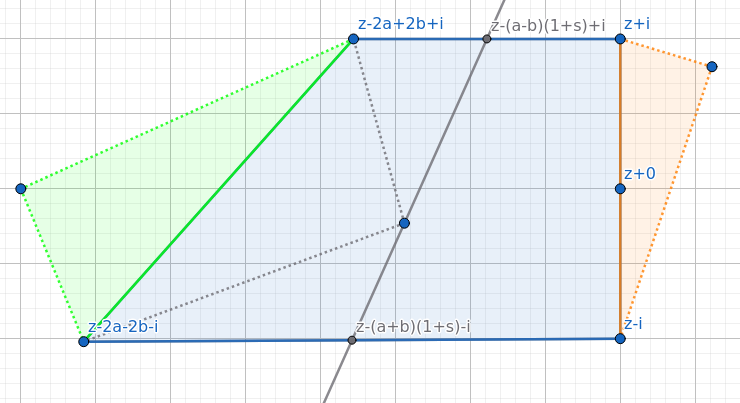
\includegraphics[width=\textwidth]{z45}
Here we have a representation of $z_4$ and $z_5$ parameterised by $s\in[-1,1]$.
We can imagine as $s$ varies, a line connecting $z_4$ and $z_5$ moving leftwards.
It will be useful for us later if we are able to take some value of $\tilde{z}$ and find the value $s$ which would a produce a line going through it.
To simplify things we can recentre by shifting by z $z \leftarrow (z-z=0)$ and let $\tilde{z} \leftarrow \tilde{z}-z$.
This operation can be undone at the end.
Moving the point $0$ along with the line towards the left gives us the point $-\alpha(1+s)$ and we can find the gradient to write the following:
\begin{align}
    (\beta(1+s)+i)t-\alpha(1+s)&=\tilde{z}=:x+iy\\
    \implies t&=y\\
    \beta(1+s)y-\alpha(1+s)&=x\\
    (1+s)(y\beta-\alpha)&=x\\
    s&=\frac{Re(\tilde{z})}{Im(\tilde{z})\beta-\alpha}-1
\end{align}
The usefulness of this formulation is that we are now able to take any arbritary point and find which region it belongs to in the above diagram.
Also given an $s$ for a $z$, we can see that $arg(z_4)-arg(z_5)$ from $s$ onwards is greater than $\pi$ and passes over the branch cut whereas when it takes on values under $s$, we have no issues with branch cuts.
We have the 3 different cases for where the origin can be relative to our value of z which we can go through one by one:

Case 3 $(Re(z)<0)$:
\begin{align}
    arg(z-(\alpha-\beta)(1+s)+i)&>arg(z+i)\\
    arg(z-(\alpha+\beta)(1+s)-i)&<arg(z-i)\\
    \implies arg(z_4)-arg(z_5)&>arg(z+i)-arg(z-i)\\
    &>\pi
\end{align}

Case 4 $(\frac{Re(0-z)}{Im(0-z)\beta-\alpha}>2\implies\frac{Re(z)}{\alpha+Im(z)\beta}>2)$:
\begin{align}
    arg(z-(\alpha-\beta)(1+s)+i)&<arg(z-2(\alpha-\beta)+i)\\
    arg(z-(\alpha+\beta)(1+s)-i)&>arg(z-2(\alpha+\beta)-i)\\
    \implies arg(z_4)-arg(z_5)&<arg(z-2(\alpha-\beta)+i)-arg(z-2(\alpha+\beta)-i)\\
    &<\pi
\end{align}

Case 5 $(s+1:=\frac{Re(z)}{\alpha+Im(z)\beta}\in[0,2])$:
\begin{align}
    s\in[-1,1] &\implies\\
    u\in[0,s+1] &\implies arg(z-(\alpha-\beta)u+i)-arg(z-(\alpha+\beta)u-i)\leq\pi\\
    s+1<u\leq2 &\implies arg(z-(\alpha-\beta)u+i)-arg(z-(\alpha+\beta)u-i)>\pi
\end{align}

From these 3 cases, we can come up with a correction using the following:
\begin{align}
    s &= max\{0, min\{\frac{Re(z)}{\alpha+Im(z)\beta},2\}\}-1\\
    \int_{-1}^1P_k(u)log(\frac{z_4}{z_5})du &=\int_{-1}^sP_k(u)(log(z_4)-log(z_5))du\\
    &+\int_s^1P_k(u)(log(z_4)-log(z_5)-2\pi i)du\\
    &=\int_{-1}^1P_k(u)(log(z_4)-log(z_5))du-2\pi i\int_s^1P_k(u)du\\
    &=\int_{-1}^1P_k(u)(log(z_4)-log(z_5))du-2\pi iC_{k+1}^{(-1/2)}(s)\\
    \int_{-1}^1C_2(s)ds &= -2\pi iC_{k+1}^{(-1/2)}(s)
\end{align}

This gives our final expression for $q_k$:
$$q_k=L_k(\frac{z-i}{\alpha-\beta}-1)-L_k(\frac{z-i}{\alpha+\beta}-1)
+2\delta_{k0}log(\frac{\alpha-\beta}{\alpha+\beta})-2\pi i C_{k+1}^{(-1/2)}(s)$$

\subsubsection{Case 4: $k=0$}
For this case we are considering how to solve the following:
\begin{align}
    \tilde{s}_{0j} &= \int_{-1}^1\frac{P_j(t)}{\alpha+\beta t}s_0(\tilde{z}_t)dt\\
    &= \int_{-1}^1\frac{P_j(t)}{\alpha+\beta t}log(\frac{\tilde{z}_t+1}{\tilde{z}_t-1})dt
\end{align}
This is difficult to find a closed form solution for, especially for all values of $j$.
We will later be forced into solving this problem with the use of dilogarithms, but we can do it in a way where we only have to do this once rather than for every value of $j$.

We can do the use the fact that we are able to compute all $r_j=s_{0j}$ to help us compute $\tilde{s}_{0j}$.
It is easy to see the relation between $s_{0j}$ and $\tilde{s}_{0j}$ as:
\begin{align}
    j>0 : s_{0j}&=\int_{-1}^1P_j(t)s_0(\tilde{z}_t)dt\\
    &=\int_{-1}^1\frac{(\alpha+\beta t)P_j(t)}{\alpha+\beta t}s_0(\tilde{z}_t)dt\\
    &=\alpha \tilde{s}_{0j} + \beta(j_-\tilde{s}_{0j-1}+j_+\tilde{s}_{0j+1})\\
    j=0 : s_{00}&=\alpha\tilde{s}_{00}+\beta\tilde{s}_{01}
\end{align}
Given a value for $\tilde{s}_{00}$ we are therefore easily able to compute all values of $\tilde{s}_{0j}$ recursively.

\subsubsection{Case 5: $j=0$}
\begin{align}
    \tilde{s}_{k0} &= \int_{-1}^1\frac{P_k(s)}{\beta(1+s)+i}s_0(\tilde{z}_s)ds\\
    &= \int_{-1}^1\frac{P_k(s)}{\beta(1+s)+i}log(\frac{\tilde{z}_s+1}{\tilde{z}_s-1})ds
\end{align}
Again for the same reasons of not being able to find a closed form solution to this we look for a $q_k$ and use this to find $\tilde{s}_{k0}$.

\begin{align}
    k>0 : q_k &= \int_{-1}^1P_k(s)s_0(\tilde{z}_s)ds\\
    &= \int_{-1}^1\frac{(\beta(1+s)+i)P_k(s)}{\beta(1+s)+i}s_0(\tilde{z}_s)ds\\
    &= (\beta+i)\tilde{s}_{k0} + \beta(k_-\tilde{s}_{k-10}+k_+\tilde{s}_{k+10})\\
    k=0 : q_0 &= (\beta+i)\tilde{s}_{00}+\beta\tilde{s}_{10}
\end{align}

Given a value of $\tilde{s}_{00}$ we are able to compute all values of $\tilde{s}_{k0}$ recursively.
Now the challenge remains to find this $\tilde{s}_{00}$.

\subsubsection{Case 6: $k,j=0,0$}
We are looking for the following:
\begin{align}
    \tilde{s}_{00}&=\int_{-1}^1\frac{s_0(\tilde{z}_t)}{\alpha+\beta t}dt=\int_{-1}^1\frac{1}{\alpha+\beta t}log(\frac{\tilde{z}_t+1}{\tilde{z}_t-1})dt\\
    &=\int_{-1}^1\frac{1}{\alpha+\beta t}log(\frac{z-it}{z-it-2(\alpha+\beta t)})dt\\
    &=\int_{-1}^1\frac{1}{\alpha+\beta t}log(\frac{z-it}{z-2\alpha-(2\beta+i)t})dt\\
    &=\int_{-1}^1\frac{log(z-it)}{\alpha+\beta t}-\int_{-1}^1\frac{z-2\alpha-(2\beta+i)t}{\alpha+\beta t}dt\\
    &=\frac{1}{\beta}(\int_{-1}^1\frac{log(z-it)}{\alpha/\beta+ t}-\int_{-1}^1\frac{z-2\alpha-(2\beta+i)t}{\alpha/\beta+t}dt)
\end{align}

We need to be able to solve solutions of the following from:
$$\int_{-1}^1\frac{log(z+ct)}{b+t}dt$$
Begin by considering decomposing $log(z+ct)\rightarrow log(\frac{z}{c}+t)+log(c)$.
Rigorously we must show that we do not cross a branch cut for all values of $t$, however, we can notice that the values of $t$ in the decomposed form is along a horizontal line.
We can assume that this interval does not cross over $0$ as our integral needs to be defined.
Because of this we can say that the whole interval either stays or crosses over the cut.
We can therefore add a correction term $(2\pi i)$ depending on $|arg(c)+arg(z/c)|$ and no correction term if this stays under $\pi$.
We can move forward by denoting as $C_3$:
\begin{align}
    \int_{-1}^1\frac{log(z+ct)}{b+t}dt&=\int_{-1}^1\frac{log(z/c+t)}{b+t}+\frac{log(c)}{b+t}dt+C_3\\
    &=\int_{-1}^1\frac{log(z/c+t)}{b+t}dt+log(c)(log(b+1)-log(b-1))+C_3
\end{align}

Now we have an integral in the form $\int_{-1}^1\frac{log(a+t)}{b+t}dt$.
In the case where $a=b$:
\begin{align}
    \int_{-1}^1\frac{log(b+t)}{b+t}dt&=\int_{b-1}^{b+1}\frac{log(t)}{t}dt\\
    u = log(t) \implies &= \int_{log(b-1)}^{log(b+1)}udu\\
    &=(log(b+1)^2-log(b-1)^2)/2
\end{align}
Otherwise if $a\neq b$:
$$\int_{-1}^1\frac{log(a+t)}{b+t}dt=\int_{b-1}^{b+1}\frac{log(a-b+t)}{t}dt$$
We know go about finding correction terms for: $log(a-b+t)\rightarrow log(a-b)+log(1+\frac{t}{a-b})$ as $a-b\in\mathbb{C}$
We have a branch crossing if for some $t\in[-1,1]$:
$$|arg(a+t)-arg(a-b)|>\pi$$
\begin{center}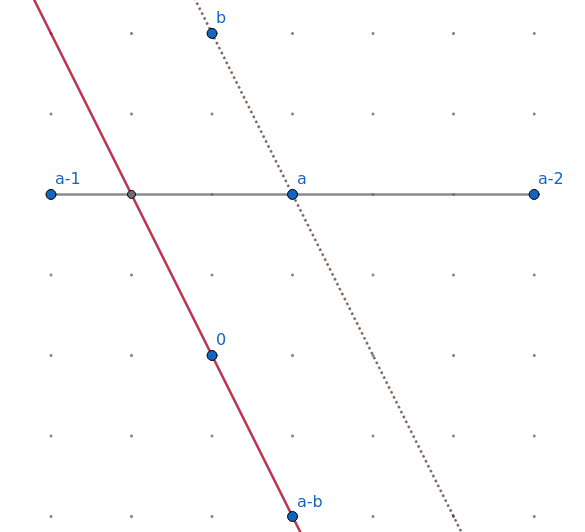
\includegraphics[width=\textwidth/2]{s00}\end{center}
Above we can see an example of $a,b$ values which results in a branch crossing over the positive side.
The red line denotes the angle at which we rotate when dividing by $a-b$.
This means that anything on the left over this line crosses the branch cut whilst anything to the right does not.
Same thing applies in the negative version where the interval of $a$ is in the negative case rotated clockwise over the branch cut.Therefore, we first have to check that a cut exists.
There are many edge cases here which I will not delve into but the rough idea is to check through the args of $a-1,a+1,a-b$ and make comparisons to determine any crossings.
With that we have handled cases where there are either no crossings or where the whole interval has crossed.
It is possible to formulate a way using trig functions to find a value of $t$ where $arg(a+t)=\pi-arg(a-b)$ in the positive case and $arg(a+t)=-\pi+arg(a-b)$ in the negative case.
let $a-b+w=a+t$ so that we have a $w$ which is a representation of the position of our intercept in the $[b-1,b+1]$ interval.
In the case where either the whole interval crosses the branch cut or none of it does we can set it to be the appropriate edge $w\in{b-1,b+1}$. This is useful since we are then able to represent the integral as follows:
\begin{align}
    \int_{-1}^1\frac{log(a+t)}{b+t}dt&=\int_{b-1}^{b+1}\frac{log(a-b+t)}{t}dt=:\int_{b-1}^{b+1}\frac{log(d+t)}{t}dt\\
    &=\int_{b-1}^{w}\frac{\pm2\pi i}{t}dt+\int_{b-1}^{b+1}\frac{log(d)+log(1+t/d)}{t}dt\\
    -u=\frac{t}{d},du=-\frac{dt}{d}:\:&=\pm2\pi ilog(\frac{w}{b-1})+log(a-b)log(\frac{b+1}{b-1})\\
    &+\int_{-\frac{b-1}{a-b}}^{-\frac{b+1}{a-b}}\frac{log(1-u)}{u}du
\end{align}
We can try to solve this using the dilogarithm function:
$$Li_2(z) = -\int_0^z\frac{log(1-u)}{u}du,\:z\in\mathbb{C}$$
We still have to be careful however since there is a branch cut for the dilogarithm function at $(1,\infty)$ at which $Li_2(z+i0^+)-Li_2(z+i0^-) = 2\pi ilog(z),\:z\in(1,\infty)$.
Ignoring edge cases which are less interesting, this can be computed by finding the x-intercept of the interval $[-\frac{b+1}{a-b},-\frac{b-1}{a-b}]$ and checking is this x intercept is part of the branch cut.
We can let $v$ denote the point at which the branch cut is crossed where $v=1$ if there is no crossing through this cut and then we can write:
$$-\int_{-\frac{b-1}{a-b}}^{-\frac{b+1}{a-b}}\frac{log(1-u)}{u}du = Li_2(-\frac{b+1}{a-b})-Li_2(-\frac{b-1}{a-b})\pm2\pi ilog(v)$$
Now that we have all the individual elements we can simply plug everything back in to compute a value for $\tilde{s}_{00}$

\subsubsection{Recovery of $s_{kj}$}
Now we have a situation where we have all values of $\tilde{s}_kj$ but no values for $s_{kj}$.
The basic idea to recover all $s_{kj}$ was by adding consecutive rows together:
$$s_{kj}=\int_{-1}^1P_j(t)s_k(\tilde{z}_t)dt=\int_{-1}^1\frac{\alpha+\beta t}{\alpha+\beta t}P_j(t)s_k(\tilde{z}_t)dt=\alpha\tilde{s}_{kj}+\beta\tilde{s}_{kj+1}$$

\section{Log kernel}
Now we move onto solving over the 2d log kernel.
This is a more useful version of the stieltjes case as we are able to use this to solve the poisson PDE:
\begin{align}
    \Delta u(\textbf{x}) &= f(\textbf{x})\:\textbf{x}\in\Omega\\
    u(\textbf{x}) &= g(\textbf{x}), \textbf{x}\in\partial\Omega\\
    \partial_nu(\textbf{x}) &= h(\textbf{x}), \textbf{x}\in\partial\Omega
\end{align}

In this section we will be trying to solve the following which is similar from the previous Stieltjes kernel:
$$L_{kj}=\int_{-1}^1(\alpha+\beta t)\int_{-1}^1P_k(s)P_j(t)log(z-it-(\alpha+\beta t)(1+s))dsdt$$
Again it is useful to simplify this to solve:
$$\tilde{L}_{kj} = \int_{-1}^1\int_{-1}^1P_k(s)P_j(t)log(z-it-(\alpha+\beta t)(1+s))dsdt$$
Recovering $L_{kj}$ is as simple as:
\begin{align}
    L_{kj}&=\alpha \tilde{L}_{kj} + \beta\int_{-1}^1\int_{-1}^1tP_j(t)P_k(s)log(z-it-(\alpha+\beta t)(1+s))dsdt\\
    j=0 &\implies L_{k0}=\alpha\tilde{L}_{k0}+\beta\tilde{L}_{k1}\\
    j>0 &\implies L_{kj}=\alpha\tilde{L}_{kj}+\beta(\frac{j}{2j+1}\tilde{L}_{kj}+\frac{j+1}{2j+1}\tilde{L}_{kj})
\end{align}

\subsection{Useful rearrangements}
Even with this simplification we will see that there are further useful simplifications we can do to uncover the recurrence relations.
The motivation is that we need some sort of recurrence to relate to this log transform and a suitable relation to use is $L_k(z):=\int_{-1}^1P_k(s)log(z-s)ds$.
However, in order to use this we need to bring $L_{kj}$ into a similar format:
\begin{align}
    log(z-it-(\alpha+\beta t)(1+s))&=log((\alpha+\beta t)\frac{z-it}{\alpha+\beta t}-1-s)\\
    &=log(\alpha+\beta t)+log(\frac{z-it}{\alpha+\beta t}-1-s)\\
    &=log(\alpha+\beta t)+log(\tilde{z}_t-s)
\end{align}
Now integrating over $s$ allows us to use the $L_k$ recurrences.
Plugging this into our original equation for $\tilde{L}_{kj}$ denoting $b_{kj}=P_k(s)P_j(t)$ for ease:
\begin{align}
    \tilde{L}_{kj}&=\int_{-1}^1\int_{-1}^1b_{kj}log(z-it-(\alpha+\beta t)(1+s))dsdt\\
    &=\int_{-1}^1\int_{-1}^1b_{kj}(log(\alpha+\beta t)+log(\tilde{z}_t-s))dsdt\\
    &=\int_{-1}^12P_j(t)log(\alpha+\beta t)\delta_{k0}dt+\int_{-1}^1P_j(t)L_k(\tilde{z}_t)dt\\
    &=\int_{-1}^12P_j(t)log(\alpha+\beta t)\delta_{k0}dt+L_{kj}^1(z)\\
    O_{kj}^1:&=\tilde L_{kj}-L_{kj}^1=2\int_{-1}^1P_j(t)log(\alpha+\beta t)\delta_{k0}dt\\
    &=2\delta_{k0}\int_{-1}^1P_j(t)(log(\beta)+log(\frac{\alpha}{\beta}+t))dt\\
    &=2\delta_{k0}(2log(\beta)\delta_{j0}+\begin{cases}
	\int_{-1}^1P_j(t)log(\frac{\alpha}{\beta}-t)dt=L_j(\alpha/\beta),&j\text{ even}\\
	\int_{-1}^1-P_j(t)log(\frac{\alpha}{\beta}-t)dt=-L_j(\alpha/\beta),&j\text{ odd}
    \end{cases})
\end{align}
Breaking this down gives us the following:
$$
O_{kj}^1=\begin{cases}
    4log(\beta)+2L_0(\alpha/\beta),&k,j=0,0\\
    2L_j(\alpha/\beta),&k=0,j>0,j\text{ even}\\
    -2L_j(\alpha/\beta),&k=0,j>0,j\text{ odd}
\end{cases}
$$
The usefulness of this is that we can now convert between solving recurrences on $\tilde L_{kj}$ and $L_{kj}^1$.
We can attempt a similar thing if we want to integrate over the $t$ instead:
\begin{align}
    log(z-it-(\alpha+\beta t)(1+s))&=log(z-it-\alpha(1+s)-t\beta(1+s))\\
    &=log(z-(\beta(1+s)+i)t-\alpha(1+s))\\
    &=log((\beta(1+s)+i)(\frac{z-\alpha(1+s)}{\beta(1+s)+i}-t))\\
    &=log((\beta(1+s)+i)(\tilde{z}_s-t))\\
    &=log(\beta(1+s)+i)+log(\tilde{z}_s-t)+C(s,t)\\
    \text{where }&C(s,t)\text{ branch correction term}
\end{align}
Plugging back into equation for $\tilde L_{kj}$ gives:
\begin{align}
    \tilde L_{kj}&=l\int_{-1}^1\int_{-1}^1b_{kj}log(z-it-(\alpha+\beta t)(1+s))dsdt\\
    &=\int_{-1}^1\int_{-1}^1b_{kj}(log(\beta(1+s)+i)+C(s,t))+b_{kj}log(\tilde{z}_s-t)dsdt\\
    &=2\delta_{j0}\int_{-1}^1P_k(s)(log(\beta)+log(\frac{\beta+i}{\beta}+s))ds+\int_{-1}^1P_k(s)L_j(\tilde z_s)ds\\
    &+\int_{-1}^1\int_{-1}^1b_{kj}C(s,t)dtds\\
    &=4log(\beta)\delta_{j0}\delta_{k0}+2\delta_{j0}(\begin{cases}
	L_k(\frac{\beta+i}{\beta}),&k\text{ even}\\
	-L_k(\frac{\beta+i}{\beta}),&k\text{ odd}\\
    \end{cases}) + L_{kj}^2\\
    &+\int_{-1}^1\int_{-1}^1b_{kj}C(s,t)dtds\\
    O_{kj}^2:&=\tilde L_{kj}-L_{kj}^2
\end{align}

This is where we run into an issue of branch cuts.
We will see how to deal with these and decompose $log((\beta(1+s)+i)\tilde{z}_s)$.
With our initial expression $log(z-it-(\alpha+\beta t)(1+s)$ we can rearrange into $log(z-\alpha(1+s)-(\beta (1+s)+i)t)$.
Fixing $s$, shows that $t$ parameterises a diagonal line on the complex plane in the direction $\beta(1+s)+i$ centered on $z-(1+s)\alpha$ as you can see from the diagram below.

\begin{center}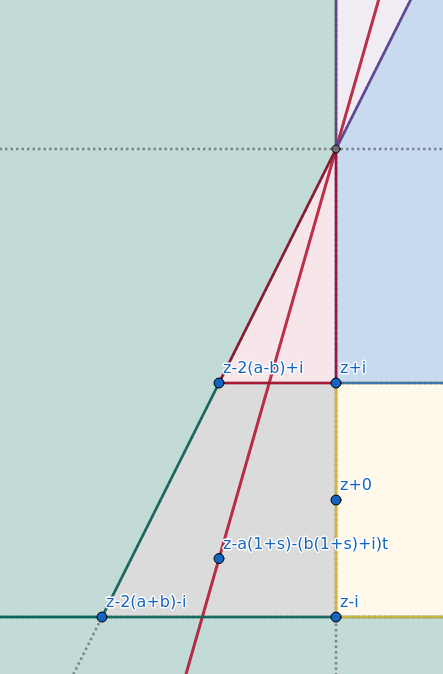
\includegraphics[width=0.75\textwidth]{ok2}\end{center}
It is possible to think of changing the value of $s$ as moving the line while it pivots around that intersection.
It is simple to compute the value of that intersection and establish cases for computing branch cuts depending on our value of $z$.
We can do this by taking two values $s$, $s'$ and trying to find $t$ such that the real component is the same:
\begin{align}
    Re(z)-\alpha(1+s)-\beta(1+s)t&=Re(z)-\alpha(1+s')-\beta(1+s')t\\
    -\alpha s-\beta st&=-\alpha s'-\beta s't\\
    \alpha(s'-s)&=\beta(s-s')t \implies t=-\frac{\alpha}{\beta}
\end{align}
Also, it is neccessary to compute a value of "$s$" of the origin relative to $z$ to reason about which case we should follow:
\begin{align}
    z-\alpha(1+s^*)-(\beta(1+s^*)+i)t&=0\\
    Im(z)-t=0 &\implies t=Im(z)\\
    Re(z)-(\alpha+\beta t)(1+s^*)&=0\\
    \frac{Re(z)}{\alpha+\beta t}=\frac{Re(z)}{\alpha+\beta Im(z)}&=s^*+1
\end{align}
To consider cases of branch cuts, we think about points where we can place the origin relative to this $z$.
Since we cannot have our $z$ in the trapezium, we will restrict ourselves to placing the origin in areas such that the $z$ is outside the trapezium.
Therefore we cannot place our origin in this greyed out region.
\subsubsection{Case 1: $Im(z)>1$}
\begin{align}
    Im(z)>1 &\implies arg(z) \in (0,\pi), \: arg(b+(1+s)i) \in (0,\frac{\pi}{2})\\
    &\implies arg(z)-arg(b+(1+s)i) > 0-\frac{\pi}{2} > -\pi\\
    \text{and }& arg(z)-arg(b+(1+s)i)<\pi-0<\pi
\end{align}

\subsubsection{Case 2: $s^*>1$ and $Im(z)\in[-\frac{\alpha}{\beta},1]$}
TODO: Can use proof similar to case 5.
In this case we have the origin in the left green region.
This means that no paths crosses the branch cut and if at all we cross in the positive real numbers, which trivially lets us infer there is no branch cut issues here

\subsubsection{Case 3: $Im(z)<-\frac{\alpha}{\beta}$ and $Re(z)>0$}
TODO: Show proof that there is no branch cut crossing here

\subsubsection{Case 4: $Re(z)<0$ and $Im(z)\in(-1,1)$}
We have that for all $s$, the integral crosses the branch cut at $t^*=Im(z)$.
Since the operation of dividing by $b(1+s)+i$ rotates the integral onto a flat line, we have that for all $s$, each integral is lifted over the branch cut.
Therefore we compensate by the correction: $-2\pi i\mathbb{I}\{t>t^*\}$
Going back to finding out correction term we have:
\begin{align}
    \int_{-1}^1\int_{-1}^1-2\pi i\mathbb{I}\{t>t^*\}P_k(s)P_j(t)dsdt&=-2\pi i\int_{-1}^12\delta_{k0}P_j(t)\mathbb{I}\{t>t^*\}dt\\
    &=-4\delta_{k0}\pi i\int_{t^*}^1P_j(t)dt
\end{align}

\subsubsection{Case 5: $s^*\in(-1,1)$ and $Im(z)>-\frac{\alpha}{\beta}$}
TODO: Make sure earlier section explains this and link to it
Letting $x^*$ be where the line of the integral crosses the real axis:
\begin{align}
    Im(z-(\alpha+\beta t)(1+s)-it)&=0\\
    Im(z)-t=0\implies &t=Im(z)\\
    x^*=Re(z)-(\alpha+\beta Im(z))(1+s)&=(\alpha+\beta Im(z))(s^*-s)\\
    Im(z)>-\frac{\alpha}{\beta}&\implies (x^*<0 \iff s^*<s)
\end{align}
Given the earlier theorem, we have that if $s>s^*$ we can say that the whole interval for that $s$ has crossed the branch cut and therefore, we compensate with the correction:$-2\pi i\mathbb{I}\{s>s^*\}$ for all $t$.
Yields our final correction term:
\begin{align}
    \int_{-1}^1\int_{-1}^1-2\pi i\mathbb{I}\{s>s^*\}P_k(s)P_j(t)dtds&=-2\pi i\int_{-1}^12\delta_{j0}\mathbb{I}\{s>s^*\}P_k(s)ds\\
    &=-4\delta_{j0}\pi i\int_{s^*}^1P_k(s)ds
\end{align}

\subsubsection{Case 6: $Im(z)\in(-\frac{\alpha}{\beta},-1)$ and $Re(z)<0$}
This is similar to Case 5 except here we can almost think of the origin having an $s^*$ value lower than -1, meaning that all the intervals of $s$ are lifted completely above the branch crossing.
We can use the $-2\pi i$ correction for every $s,t$ in our integration:
$$\int_{-1}^1\int_{-1}^1-2\pi iP_k(s)P_j(t)dsdt=-8\pi i\delta_{k0}\delta_{j0}$$

\subsubsection{Case 7: $Im(z)<-\frac{\alpha}{\beta}$ and $s^*\in(-1,1)$}
Also similar to case 5 except reversed.
We will begin with the result from case 5:
\begin{align}
    x^*=Re(z)-(\alpha+\beta Im(z))(1+s)&=(\alpha+\beta Im(z))(s^*-s)\\
    Im(z)<-\frac{\alpha}{\beta}&\implies (x^*<0 \iff s^*>s)
\end{align}
The correction term here is then $-2\pi i\mathbb{I}\{s<s^*\}$:
\begin{align}
    \int_{-1}^1\int_{-1}^1-2\pi i\mathbb{I}\{s<s^*\}P_k(s)P_j(t)dtds&=-2\pi i\int_{-1}^12\delta_{j0}\mathbb{I}\{s<s^*\}P_k(s)ds\\
    &=-4\delta\pi i\int_{-1}^{s^*}P_k(s)ds
\end{align}

\subsubsection{Case 8:  $s^*>1$ and $Im(z)<-\frac{\alpha}{\beta}$}
Also similar to case 5:
\begin{align}
    x^*=Re(z)-(\alpha+\beta Im(z))(1+s)&=(\alpha+\beta Im(z))(s^*-s)\\
    &>(\alpha+\beta Im(z))(1-s)\\
    (\alpha+\beta Im(z))<0 \text{ and } 1-s>0 &\implies x^*<0
\end{align}
This means the whole interval must be corrected by $-2\pi i$ for each point and $-8\pi i\delta_{k0}\delta_{j0}$ for the whole interval like in case 6.

\subsubsection{Case 9: $|s^*|<1$ and $|Im(z)|<1$}
Combining the logic in the earlier cases we have that the branch cut correction here is just $-2\pi i\mathbb{I}\{s>s^*\}\mathbb{I}\{t>t^*\}$.
This gives us the total correction:
$$-2\pi i(\int_{s^*}^1P_k(s)ds)(\int_{t^*}^1P_j(t)dt)$$

\subsection{Recurrences}
\subsubsection{Note on notation}
We will be continuing with the convention of representing the 3 term recurrence constants as follows:
$$tP_j(t)=j_-P_{j-1}(t)+j_+P_{j+1}$$
To add onto this we will be using a recurrence relation of $L_k(z)$ as follows:
\begin{align}
    zL_k(z) &= \frac{k-1}{2k+1}L_{k-1}(z)+\frac{k+2}{2k+1}L_{k+1}(z)+\lambda_k(z)\\
    :&= k_-^LL_{k-1}(z)+k_+^LL_{k+1}(z)+\lambda_k(z)\\
    \lambda_k(z) &= \begin{cases}
	(z-1)log(z-1)+(z+1)log(z+1),&k=0\\
	-2/3,&k=1\\
	0,&\text{otherwise}
    \end{cases}
\end{align}
\subsubsection{Case 1: $k,j>1$}
For this case we can use either offsets but we go with working in $L_{kj}^1$
\begin{align}
    zL_{kj}^1 &= \int_{-1}^1zP_j(t)L_k(\tilde{z}_t)dt\\
    &= \int_{-1}^1(z-\alpha-(\beta+i)t)P_j(t)L_k(\tilde{z}_t)dt
    +\int_{-1}^1(\alpha+(\beta+i)t)P_j(t)L_k(\tilde{z}_t)dt\\
    &= \int_{-1}^1(\alpha+\beta t)\frac{z-it-(\alpha+\beta t)}{\alpha+\beta t}P_j(t)L_k(\tilde{z}_t)dt
    +\int_{-1}^1(\alpha+(\beta+i)t)P_j(t)L_k(\tilde{z}_t)dt\\
    &= \int_{-1}^1(\alpha+\beta t)P_j(t)\tilde{z}_tL_k(\tilde{z}_t)dt
    +\int_{-1}^1(\alpha+(\beta+i)t)P_j(t)L_k(\tilde{z}_t)dt\\
    &= \int_{-1}^1(\alpha+\beta t)P_j(t)(k_-^LL_{k-1}(\tilde{z}_t)+k_+^LL_{k+1}(\tilde{z}_t)-\frac{2}{3}\delta_{k1})dt\\
    &+\alpha L_{kj}^1+(\beta+i)(j_-L_{kj-1}^1+j_+L_{kj+1}^1)\\
    &=\alpha(k_-^LL_{k-1j}^1+k_+^LL_{k+1j}^1)+
    \beta(k_-^Lj_-L_{k-1j-1}^1+k_-^Lj_+L_{k-1j+1}^1\\
    &+k_+^Lj_-L_{k+1j-1}^1+k_+^Lj_+L_{k+1j+1}^1)+\alpha L_{kj}^1+(\beta+i)(j_-L_{kj-1}^1+j_+L_{kj+1}^1)\\
    &-\frac{2\beta}{3}\frac{1}{3}2\delta_{k1}\delta_{j1}
\end{align}

\subsubsection{Case 2: $k=1$}
\begin{align}
    zL_{0j}^2&=\int_{-1}^1zL_j(\tilde z_s)ds\\
    &=\int_{-1}^1(\beta(1+s)+i)\tilde z_sL_j(z_s)ds+\int_{-1}^1\alpha(1+s)L_j(\tilde z_s)ds\\
    &=\int_{-1}^1(\beta(1+s)+i)(j_-^LL_{j-1}(\tilde z_s)+j_+^LL_{j+1}(\tilde z_s)-\frac{2}{3}\delta_{j1})ds\\
    &+\int_{-1}^1\alpha(1+s)L_j(\tilde z_s)ds\\
    &=(\beta+i)(j_-^LL_{0j-1}^2+j_+^LL_{0j+1}^2-\frac{4\delta_{j1}}{3})+\beta(j_-^LL_{1j-1}^2+j_+^LL_{1j+1}^2)\\
    &+\alpha L_{0j}^2+\alpha L_{1j}^2\\
\end{align}

\subsubsection{Case 3: $j=1$}
\begin{align}
    zL_{k0}^1&=\int_{-1}^1zL_k(\tilde z_t)dt\\
    &=\int_{-1}^1(\alpha+\beta t)\tilde z_tL_k(\tilde z_t)dt+\int_{-1}^1(\alpha+(\beta+i))tL_k(\tilde z_t)dt\\
    &=\int_{-1}^1(\alpha+\beta t)(k_-^LL_{k-1}(\tilde z_s)+k_+^LL_{k+1}(\tilde z_s)-\frac{2}{3}\delta_{k1})dt\\
    &+\int_{-1}^1(\alpha+(\beta+i))tL_k(\tilde z_t)dt\\
    &=\alpha(k_-^LL_{k-10}^1+k_+^LL_{k+10}-\frac{4\delta_{k1}}{3})+\beta(k_-^LL_{k-11}^1+k_+^LL_{k+11})\\
    &+\alpha L_{k0}^1+(\beta+i)L_{k1}^1
\end{align}

\subsubsection{Case 4: $k,j=1,1$}
As seen earlier we can describe the $L_k$ relation for $k=0$ as:
$$zL_0(z)=2L_1(z)+\lambda_0(z)\text{ where } \lambda_0(z)=(z-1)log(z-1)+(z+1)log(z+1)$$
First its important to solve:
\begin{align}
    \int_{-1}^1(\alpha+\beta t)\lambda_0(\tilde z_t)dt&=\int_{-1}^1(z-it)log(\frac{z-it}{\alpha+\beta t})\\
    &+(z-2\alpha-(2\beta+i)t)log(\frac{z-2\alpha-(2\beta+i)t}{\alpha+\beta t})dt\\
    &=2(\alpha+\beta t)log(\alpha+\beta t)dt+\int_{-1}^1(z-it)log(z-it)\\
    &+(z-2\alpha-(2\beta+i)t)log(z-2\alpha-(2\beta+i)t)\\
\end{align}
We are able to use techniques from the earlier section TODO: reference section.
Since then we are able to find this we can now find the overall recurrence:
\begin{align}
    zL_{00}^1&=\int_{-1}^1zL_0(\tilde z_t)dt\\
    &=\int_{-1}^1(\alpha+\beta t)\tilde zL_0(\tilde z)dt+\int_{-1}^1(\alpha+(\beta+i)t)L_0(\tilde z)dt\\
    &=2\alpha L_{10}^1+2\beta L_{11}^1+\alpha L_{00}^1+(\beta+i)L_{01}^1+\int_{-1}^1(\alpha+\beta t)\lambda_0(\tilde z_t)dt
\end{align}

\subsubsection{Case 5: $k=0$}
The easiest way to solve for this is to work in $L_{kj}^1$.
We will also make use of the fact that $L_0(z)=(z+1)(log(z+1)-1)-(z-1)(log(z-1)-1)=(z+1)log(z+1)-(z-1)log(z-1)-2$.
\begin{align}
    L_{0j}^1 &= \int_{-1}^1P_j(t)L_0(\tilde z_t)dt\\
    &= \int_{-1}^1P_j(t)((\tilde z_t+1)log(\tilde z_t+1)-(\tilde z_t-1)log(\tilde z_t-1)-2)dt\\
    &= \int_{-1}^1P_j(t)(\frac{z-it}{\alpha+\beta t}log(\frac{z-it}{\alpha+\beta t})-(\frac{z-2\alpha-(2\beta+i)t}{\alpha+\beta t})log(\frac{z-2\alpha-(2\beta+i)t}{\alpha+\beta t})-2)dt\\
    &=\int_{-1}^1\frac{P_j(t)}{\alpha+\beta t}((z-it)log(\frac{z-it}{\alpha+\beta t})\\
    &-(z-2\alpha-(2\beta+i)t)log(\frac{z-2\alpha-(2\beta+i)t}{\alpha+\beta t})-2(\alpha+\beta t))dt\\
    &=\int_{-1}^1\frac{P_j(t)}{\alpha+\beta t}((z-it)log(z-it)+(z-2\alpha-(2\beta+i)t)log(z-2\alpha-(2\beta+i)t)\\
    &+2(\alpha+\beta t)(log(\alpha+\beta t)-1))dt
\end{align}
We can simplify this by trying to solve:
$$\tilde l_j= \int_{-1}^1(\alpha+\beta t)P_j(t)L_0(\tilde z_t)dt$$
Breaking it down even further we are just solving 1: $\int_{-1}^1P_j(t)log(z-it)dt = M_j(t)$ and 2:
\begin{align}
    \int_{-1}^1P_j(t)log(z-2\alpha-(2\beta+i)t)dt&=\int_{-1}^1P_j(t)log(2\beta+i)\\
    &+P_j(t)log(\frac{z-2\alpha}{2\beta+i}-t)+P_j(t)C(t)dt\\
    &= 2(2\beta+i)\delta_{j0}+L_j(\frac{z-2\alpha}{2\beta+i})+\int_{-1}^1P_j(t)C(t)dt
\end{align}
letting $x^*=Re(z)-2(\alpha+\beta)Im(z)$ i.e the value of the reals when we extend the interval to cross the real axis where the imaginary component is $0$:
$$
\int_{-1}^1P_j(t)C(t)dt = \begin{cases}
    -2\pi i\int_{Im(z)}^1P_j(t)dt,&x^*<0,\:|Im(z)|<1\\
    -4\pi i\delta_{j0},&x^*<0,\:Im(z)<-1\\ 
    0,&\text{otherwise}
\end{cases}
$$
Solving the log part of the $\tilde l_j$ is very trivial and we have seen multiple instances of this case before where we turn it into the form of $L_k$.
Now that we know how to solve for $\tilde l_j$ we can go about solving $L_{0j}^1$.
For this to work we need a value for $L_{00}^1$ to get started with the forward substitution which I will describe in a different case.
By computing $L_{01}^1=\frac{1}{\beta}(\tilde l_0-\alpha L_{00}^1)$, we can find the rest:
$$L_{0j+1}^1 = \frac{1}{j_+\beta}(\tilde l_j-\alpha L_{0j}^1-j_-\beta L_{0j-1}^1)$$

\subsubsection{Case 6: $j=0$}
In order to solve this we must first work out how to correct for a certain type of branch cut in the form of:
$$f(s)log(z-\gamma(1+s)) \rightarrow f(s)(log(\frac{z-\gamma(1+s)}{\beta(1+s)+i})+log(\beta(1+s)+i)+C(s))$$
\begin{center}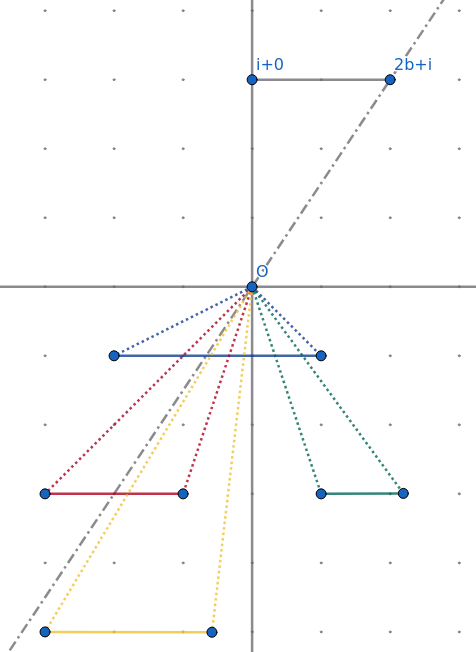
\includegraphics[width=0.5\textwidth]{bsi}\end{center}
Above is an image which shoes the interval at the top ($\beta(1+s)+i$) and a few intervals beneath the real axis in the form of $z-\gamma(1+s)$.
We have a crossing of the branch cut for some $s$ if $arg(z-\gamma(1+s))-arg(\beta(1+s)+i)<-\pi$.
Intuitively, we can see this condition will be fulfilled for some $s$ if the angle from the interval $\beta(1+s)+i$ to the interval below exceeds $\pi$.
Therefore we can find for each interval some values of $s$ where it goes from crossing the branch cut to not crossing it and vice versa depending on where the below interval is.
Above are some examples: The blue interval begins without any branch crossings but at the end of the interval ($2b+i\rightarrow z-2\gamma$), we have that the angle between these is greater than $\pi$.
Therefore, at some point there would be an $s$ where the branch cut is crossed.
We can show using some calculations that this value of $s$ is unique and that there are no cases of multiple branch crossings within the same interval.
The green interval is fine the whole way through and the red is on the other side of the branch cut the whole way through.
Finally, the yellow interval is the opposite as the blue since it begins crossed over but then returns to the "correct" side.
Caclulating which side of the branch cut the interval begins on is relatively trivial as we can just check if the value of $z$ has a positive or a negative real component.
Computing some value $s^*$ for which we have a crossing is as follows:
\begin{align}
    \lambda(\beta(1+s^*)+i)&=z-\gamma(1+s^*),\lambda\in\mathbb{C}\\
    Im:\:\lambda&=Im(z)\\
    Re:\:Im(z)\beta(1+s^*)&=Re(z)-\gamma(1+s^*)\\
    (Im(z)\beta+\gamma)(1+s^*)&=Re(z)\\
    s^*&=\frac{Re(z)}{Im(z)\beta+\gamma}
\end{align}
Since $s^*$ is defined to be the point at which a crossing occurs, we force the value of $s^*$ to be $1$ if the above calculation results in something outside of the interval $[-1,1]$ since this means that any crossings happens outside.
There is a case where $Im(z)\beta+\gamma=0$ which can be thought if as when we essentially have that there will never be a crossing.
An example of when this can happen is if $z=-i,\:\gamma=\beta$ which is where both lines move symmetrically away from the imaginary axis and stay at exactly $\pi$ away.

The easiest way to solve $\tilde L_{k0}$ is to work in $L_{kj}^2$.
\begin{align}
    L_{k0}^2 &= \int_{-1}^1P_k(s)L_0(\tilde z_s)ds\\
    &= \int_{-1}^1P_k(s)((\tilde z_s+1)log(\tilde z_s+1)-(\tilde z_s-1)log(\tilde z_s-1)-2)ds\\
    &= \int_{-1}^1P_k(s)(\frac{z-(\alpha-\beta)(1+s)+i}{\beta(1+s)+i}log(\frac{z-(\alpha-\beta)(1+s)+i}{\beta(1+s)+i})\\
    &-\frac{z-(\alpha+\beta)(1+s)-i}{\beta(1+s)+i}log(\frac{z-(\alpha+\beta)(1+s)-i}{\beta(1+s)+i})-2)ds\\
    &=\int_{-1}^1\frac{P_k(s)}{\beta(1+s)+i}((z-(\alpha-\beta)(1+s)+i)(log(z-(\alpha-\beta)(1+s)+i)\\
    &-log(\beta(1+s)+i)+C_+(s))-(z-(\alpha+\beta)(1+s)-i)(log(z-(\alpha+\beta)(1+s)-i)\\
    &-log(\beta(1+s)+i)+C_-(s))-2(\beta(1+s)+i)ds\\
    &=\int_{-1}^1\frac{P_k(s)}{\beta(1+s)+i}((z-(\alpha-\beta)(1+s)+i)(log(z-(\alpha-\beta)(1+s)+i)+C_+(s))\\
    &-(z-(\alpha+\beta)(1+s)-i)(log(z-(\alpha+\beta)(1+s)-i)+C_-(s))\\
    &2(\beta(1+s)+i)(log(\beta(1+s)+i)-1)ds
\end{align}
Where $C_+, C_-$ are correction terms for branch cuts from splitting the log.
\begin{align}
    log(z-(\alpha\mp\beta)(1+s)\pm i)&=log(\frac{z-(\alpha\mp\beta)(1+s)\pm i}{\beta(1+s)+i})+log(\beta(1+s)+i)+C_\pm\\
    s_\pm^*= \frac{Re(z\pm i)}{Im(z\pm i)\beta+(\alpha\mp\beta)}-1&=\frac{Re(z)}{Im(z)\beta\pm\beta+\alpha\mp\beta}-1=\frac{Re(z)}{Im(z)\beta+\alpha}-1\\
\end{align}
Applying the results from branch cut analysis from before we can try finding the correction $C_+,C_-$.
As we see, the values of $s^*$ are the same for both cases as long as $Im(z)<-1$ and therefore:
$$C_\pm(s)=\begin{cases}
    2\pi i\mathbb{I}\{s>s^*\}\mathbb{I}\{Im(z)\pm1<0\},&Re(z)>0\\
    2\pi i\mathbb{I}\{s<s^*\}\mathbb{I}\{Im(z)\pm1<0\},&Re(z)<0
\end{cases}$$
Going back to our original expression we do the same trick as earlier where we define and solve:
$$\tilde l_k^2=\int_{-1}^1(\beta(1+s)+i)P_k(s)L_0(\tilde z_s)ds$$
Solving $l_k^2$ can be done by solving its individual components:
$$\int_{-1}^1P_k(s)log(z-(\alpha\mp\beta)(1+s)\pm i)ds=2log(\alpha\mp\beta)\delta_{k0}
+L_k(\frac{z}{\alpha\mp\beta}\pm i-1)$$
The correction terms can be trivially attained by adjusting the bounds of the legendre polynomial integrals and multiplying by a constant factor e.g $\int_s^1P_k(s)ds$
We follow the same protocal as before to obtain all $L_{k0}^2$ by starting the forward substitution with $L_{00}^2$ and $L_{10}^2=\frac{1}{\beta}(\tilde l_0^2-(\beta+i)L_{00}^2)$:
$$L_{k+10}^2=\frac{1}{k_+\beta}(\tilde l_k^2-(\beta+i)L_{k0}^2-k_-\beta L_{k-10}^2)$$

\subsubsection{Case 7: $k,j=0,0$}
In this section chosing between $L_{kj}^1$ and $L_{kj}^2$ is very arbritary so we simply pick the former:
$$L_{00}^1 = \int_{-1}^1L_0(\tilde z_t)dt$$

\section{Transformation}
Up until now, we have been working in very fixed regions using the least amount of degrees of freedom possible for parameterisation.
In this section we will explore how to resize and move around our region so we can achieve more complex structures by computing over smaller regions.
We will be revisting the stieltjes over a square:
$$s_{kj} = \int_{-1}^1\int_{-1}^1\frac{P_k(s)P_j(t)}{z-(s+it)}dsdt$$
Let us also recall the way we approach function decomposition onto our function bases:
$$f\circ Q(\textbf{x})=\Sigma_{k,j}c_{k,j}b_{kj}(\textbf{x}),\:b_{kj}(\textbf{x})=P_k(\textbf{x}_0)P_j(\textbf{x}_1)$$
The transformations which are available to us are operations which we can perform on $z$ which lets us alter the region we are integrating over which is parameterised as $s+it$.

\subsection{Translation}
If we want to translate the region of interest from $[-1,1]\times[-1,1]$ to $[x-1,x+1],[y-1,y+1]$, we need to change the region to $x(s,t)+x+i(t+y)$ where $x(s,t)$ is a function that takes values from the space of $s,t$ and gives out where $s$ should be based on what shape we are working with.
This lets us rewrite the expression in the kernel as $(z-x-iy)-(x(s,t)+it)$.
Since we do not interfere with the formula of the kernel, this works for both stieltjes and for log kernels.
Therefore the same recursion rules but with a different value of $z$ gives us this.

\subsection{Scaling and Rotation}
\subsubsection{Stieltjes kernel}
The kernel of the stieltjes integral is in the form of $z-x(s,t)-it$ in the general case.
This means that we can multiply this thie region of $x(s,t)-it$ by $\lambda\in\mathbb{c}$
The real component of this value contributes to the scaling and the complex component the rotation.
We can therefore rewrite the scaled $s_{kj}(z)$ as $\frac{1}{\lambda}s_{kj}(\frac{z}{\lambda})$
\subsubsection{Log kernel}
We can apply a similar sort of technique as before as we are trying to go from:
\begin{align}
    Log(z-(\alpha+\beta t)(1+s)-it)&\rightarrow Log(z-\lambda((\alpha+\beta t)(1+s)-it))\\
    &= Log(\lambda(\frac{z}{\lambda}-(\alpha+\beta t)(1+s)-it))
\end{align}
Sadly, in order to split this we must yet again consider branch cuts since $\lambda\in\mathbb{C}$

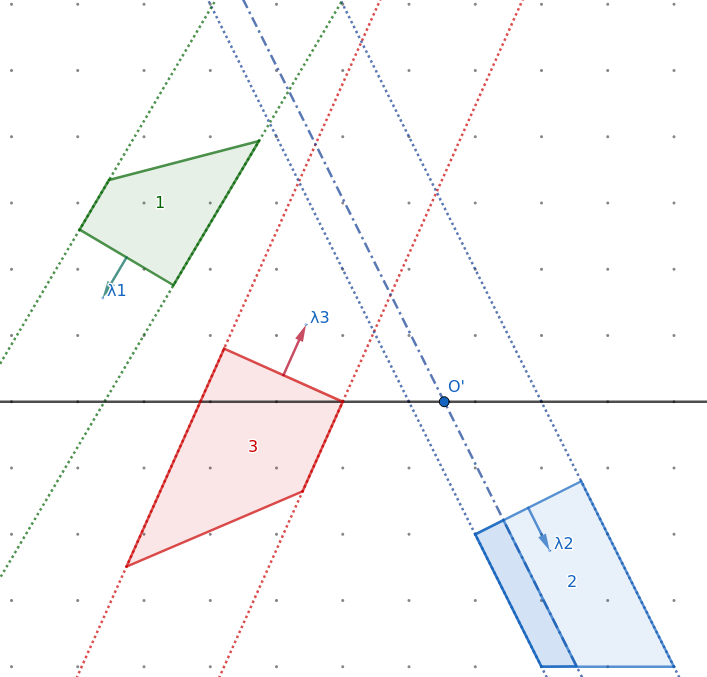
\includegraphics[width=\textwidth]{lscale}

We can see in this above image 3 different examples for various transformations on different values of $\lambda$ centered around different values of $z$.
We have that by dividing by $\lambda$, the trapeziums will be rotated by that angle and will end up with the $\lambda$ vector pointing with arg 0.
Note that this is a more general version of the linear log interval transformations which were made.
Going through the above examples, the green trapezium is to be rotated anticlockwise over the branch cut if the origin is to the right of the x intersection (if it was to its left it wouldn't need to rotate as far as to cross it).
The red one is a little trickier, since it exists currently on a branch cut, it is difficult to work with.
In fact it the simplest way to tackle these are to split them up into two shapes and work on each independently.
To do this we can extend into a rectangle, solve the rectangle as two trapeziums split along the real axis and remove the excess trapeziums and rectangles to obtain our original shape.
The blue trapezium shows what happens if we have the origin positioned where part of the trapezium when rotated is lifted over and a section which is not.
Correction is only applied to the area which is lifted past.
This prompts us to be able to find a value for $t$ which represents the split which can be drawn from the origin if it falls between the two parallel lines.
The value of $t$ begin outside ($-1,1$) means that we have a case where the parallel lines are both have real axis intercepts on the same side as the origin.
\begin{align}
    \text{let: }x=(\alpha+\beta t)(1+s)\\
    \text{We need: }z-\mu-\lambda((\alpha+\beta t)(1+s)+it)&=0=z-\mu-\lambda(x+it)\\
    Re:\:Re(z-\mu)-xRe(\lambda)+tIm(\lambda)&=0\\
    Im:\:Im(z-\mu)-xIm(\lambda)-tRe(\lambda)&=0\\
    \begin{bmatrix}
	-Re(\lambda)&Im(\lambda)\\
	-Im(\lambda)&-Re(\lambda)\\
    \end{bmatrix}
    \begin{bmatrix}x\\t\end{bmatrix}
    &=\begin{bmatrix}-Re(z-\mu)\\-Im(z-\mu)\end{bmatrix}\\
    \text{non singular: }\lambda\neq 0\implies Re(\lambda)^2+Im(\lambda)^2&>0
\end{align}

\section{Boundary Conditions}
Now we have all the tools to be able to solve the poisson equation: $\Delta u=f$ for any arbritary function $f$ by convolving its green's function ($\frac{1}{2\pi}ln|x-y|$) over the target function $f$.
This essentially gives us a function that satisfies $\Delta u(x)=f(x)$ over a 2d domain but nothing else.
What is useful to be able to do is to be able to set boundary conditions on this problem.
Let the result we obtain be $u_p$. As well as:
\begin{align}
    u_p(x)&=g_p(x),\:x\in\partial\Omega\\
    \frac{\partial u_p(x)}{\partial n}&=h_p(x),\:x\in\partial\Omega
\end{align}
We wish for a solution where $u(x)=g(x)\text{ and }\partial_nu(x)=h(x)$ on the boundary.
The idea here is to solve a homogeneous pde:
\begin{align}
    \Delta u(x)&=0, x\in\Omega\\
    u(x)&=g(x)-g_p(x),\\
    \partial_nu(x)&=h(x)-h_p(x),x\in\partial\Omega
\end{align}
Therefore the solution $u(x)+u_p(x)$ will satisfy $\Delta(u+u_p)=f$ as well as the desired boundary conditions.
Now all we need is to come up with a way to find solutions to the problem $\Delta u=0$ for any given boundary condition.
\subsection{Boundary element method}
We begin with our initial equation and multiply test function $w$ to get a weak solution:
\begin{align}
    \Delta u=0&\implies \int_\Omega w\Delta u=0\\
    \int_\Omega w\Delta u&=\int_{\partial\Omega}w\partial_nu-\int_\Omega(\nabla u)\cdot(\nabla w)\\
    &=\int_{\partial\Omega}w\partial_nu-(\int_{\partial\Omega}u\partial_nw-\int_\Omega u\Delta w)\\
    \int_\Omega u\Delta w&=\int_{\partial\Omega}u\partial_nw-w\partial_nu
\end{align}
If we let our $w$ be the greens function i.e $\Delta w_y(x) = \delta(x,y)$, we can simplify the above down:
$$y\in\Omega,\:\int_\Omega u\Delta w_y=u(y)=\int_{\partial\Omega}u\partial_nw_y-w_y\partial_nu$$
As you can see we have an expression for the solution which is in the form of an integral along the boundary.
Firstly, we need an expression for $\partial_nw_y = \partial_n\frac{1}{2\pi}ln|x-y|$:
\begin{align}
    \nabla ln|x-y|&=\nabla ln(\sqrt{(x_i-y_i)^2})=\nabla\frac{1}{2}ln((x_i-y_i)^2)\\
    (\nabla ln|x-y|)_i &=\frac{x_i-y_i}{|x-y|^2}\\
    \partial_n ln|x-y| &= \hat n\cdot\nabla ln|x-y| = \frac{\hat n\cdot(x-y)}{|x-y|^2} = \frac{\hat n\cdot x}{|x-y|^2}-\frac{\hat n\cdot y}{|x-y|^2}
\end{align}
Since we have boundaries which are straight lines we have that over each line $i,\hat n_i$ stays constant and therefore so does $\hat n\cdot y$.
If we are able to integrate over a single line then we can sum up the results to get the entire boundary.
We will revist the case of a stieltjes kernel over a simple interval but decompose $z=x+iy$ to see what happens.
\begin{align}
    S_k(z)=\int_{-1}^1\frac{P_k(s)}{z-s}ds&=\int_{-1}^1\frac{P_k(s)}{x-s+iy}ds\\
    &=\int_{-1}^1P_k(s)\frac{x-s-iy}{(x-s)^2+y^2}ds\\
    Re(S_k(z))&=\int_{-1}^1P_k(s)\frac{Re(z)-s}{|z-s|^2}ds\\
    -Im(S_k(z))&=\int_{-1}^1P_k(s)\frac{Im(z)}{|z-s|^2}ds\\
    S_k(z)^*=Re(S_k(z))-Im(S_k(z))i&=\int_{-1}^1P_k(s)\frac{z-s}{|z-s|^2}ds
\end{align}
We can apply this to the problem of finding the integral of $u\partial_nw$ across an edge as follows:
\begin{align}
    \int_{\partial\Omega_j}u\partial_nw_z&=\int_{\partial\Omega_j}u\frac{\hat n\cdot(x-z)}{2\pi|x-z|^2}dx
    =\frac{\hat n}{2\pi}\cdot\int_{\partial\Omega_j}\frac{u(x-z)}{|x-z|^2}dx\\
    &=\frac{\hat n}{2\pi}\cdot\int_{-1}^1u\frac{\mu+\lambda s-z}{|\mu+\lambda s-z|^2}ds
    =-\frac{\hat n}{2\pi|\lambda|^2}\cdot\lambda\int_{-1}^1u\frac{\frac{z-\mu}{\lambda}- s}{|\frac{z-\mu}{\lambda}-s|^2}ds\\
    &=-\frac{\hat n}{2\pi|\lambda|^2}\cdot\Sigma_kc_k\lambda\int_{-1}^1P_k(s)\frac{\tilde z- s}{|\tilde z-s|^2}ds\\
    &=-\frac{\hat n}{2\pi|\lambda|^2}\cdot\Sigma_kc_k\lambda S_k(z)^*
\end{align}
Let $\tilde z = \frac{z-\mu}{\lambda}$ be normalised $z$.
Th other component of the greens identity was $w_y\partial_nu$.
Given boundary conditions $\partial_nu$ on our $\partial\Omega$, we have a transformed log line kernel which we already know how to solve.
\section{Larger Meshes}
We can add together results from individual triangles to get the result of a convolution over more complicated regions.
Given that we are approximating functions to an order of $p$ which results in $p^2$ basis functions, we have that for a single value of $z$ we have $O(p^2)$ operation.
If we naively add up all $n$ shapes, we have $O(np^2)$ and now it has started to increase in size.
\end{document}

